\begin{figure}[!t]
\centering
\small

\begin{tabular}{c@{\hskip 7ex}c}
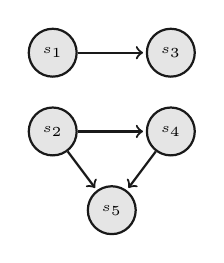
\begin{tikzpicture}[shorten >=1pt,->,scale=0.5]  
        \tikzstyle{sentence}=[circle,thick,draw=black!90,fill=black!10,minimum size=2mm]
	\tikzstyle{entity}=[circle,thick,draw=black!90,fill=black!10,minimum size=2mm]
        \tikzstyle{edge}=[draw=black!90, thick]
       \begin{scope}
       
         \node [sentence] (s1) at (0,4) {\tiny{$s_1$}};
         \node [sentence] (s2) at (0,2) {\tiny{$s_2$}};
         \node [sentence] (s3) at (3,4) {\tiny{$s_3$}}; 
         \node [sentence] (s4) at (3,2) {\tiny{$s_4$}}; 
         \node [sentence] (s5) at (1.5,0) {\tiny{$s_5$}}; 
 
 		\path[edge] (s1) edge [above] node[font=\tiny]{} (s3);
 		\path[edge] (s2) edge [above] node[font=\tiny]{} (s4);
		\path[edge] (s2) edge [above] node[font=\tiny]{} (s5);
 		\path[edge] (s4) edge [above] node[font=\tiny]{} (s5);
               
        \end{scope}        
      \end{tikzpicture}

&      

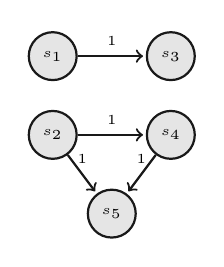
\begin{tikzpicture}[shorten >=1pt,->,scale=0.5]  
        \tikzstyle{sentence}=[circle,thick,draw=black!90,fill=black!10,minimum size=2mm]
	\tikzstyle{entity}=[circle,thick,draw=black!90,fill=black!10,minimum size=2mm]
        \tikzstyle{edge}=[draw=black!90, thick]
       \begin{scope}
       
         \node [sentence] (s1) at (0,4) {\tiny{$s_1$}};
         \node [sentence] (s2) at (0,2) {\tiny{$s_2$}};
         \node [sentence] (s3) at (3,4) {\tiny{$s_3$}}; 
         \node [sentence] (s4) at (3,2) {\tiny{$s_4$}}; 
         \node [sentence] (s5) at (1.5,0) {\tiny{$s_5$}}; 
 
 		\path[edge] (s1) edge [above] node[font=\tiny]{1} (s3);
 		\path[edge] (s2) edge [above] node[font=\tiny]{1} (s4);
		\path[edge] (s2) edge [above] node[font=\tiny]{1} (s5);
 		\path[edge] (s4) edge [above] node[font=\tiny]{1} (s5);
               
        \end{scope}        
      \end{tikzpicture}
\\ \scriptsize{$P_u^{ER}$} & \scriptsize{$P_w^{ER}$}

\end{tabular}
\caption{$P_u^{ER}$: unweighted and $P_w^{ER}$: weighted projection graphs. In weighted projection all edge weights are equal to one because all sentences share one entity.}

\label{f:entity_projection}
\end{figure}